\documentclass{article}
\usepackage[margin=1in]{geometry} % For setting page margins
\usepackage{amsmath}
\usepackage{amssymb} % For math symbols and equations
\usepackage{graphicx} % For including images
\usepackage{hyperref} 
\usepackage{enumitem}
\usepackage{float}
\usepackage{listings}
\usepackage{xcolor}
\usepackage{caption}

\renewcommand{\thesection}{\arabic{section}.}
\renewcommand{\thesubsection}{(\alph{subsection})}

\lstdefinestyle{matlabstyle}{
    language=Matlab,              % Specify the language
    basicstyle=\ttfamily\footnotesize\color{black}, % Code font
    keywordstyle=\color{blue}\bfseries, % Keywords in blue
    stringstyle=\color{orange},    % Strings in green
    commentstyle=\color{magenta}, % Comments in magenta
    numbers=left,                 % Line numbers on the left
    numberstyle=\tiny\color{black},% Line number style
    stepnumber=1,                 % Line number increment
    breaklines=true,              % Line breaking
    frame=single,                 % Border around code
    backgroundcolor=\color{white},
    tabsize=4,                    % Tab size
    showstringspaces=false,       % Don't show spaces in strings
}

\begin{document}

\title{
    \begin{tabular}{@{}l@{}}
        \textbf{Class:} Robust Multivariate Control \\
        \textbf{Professor:} Dr. Sean Humbert \\
        \textbf{TAs:} Santosh Chaganti \\
        \textbf{Student:} Steve Gillet \\
        \textbf{Date:} \today \\
        \textbf{Assignment:} Homework 7
    \end{tabular}
}

\author{}
\date{}

\maketitle

\section{}
\textit{In this problem you will analyze the robustness properties of a F-16 equipped with a lateral regulator. We consider the lateral dynamics $(\beta, \phi, p, r)$ augmented with aileron and rudder actuator dynamics $\left(\delta_a, \delta_r\right)$ and a washout filter $\left(x_w\right)$ in the yaw channel. The state vector of the augmented dynamics is $\left(\beta, \phi, p, r, \delta_a, \delta_r, x_w\right)$. The outputs of the model include $\left(r_w, p, \beta, \phi\right)$ where $r_w$ is the washed out yaw rate. Assume a static controller $u = K e$ where
\[
K = \begin{bmatrix}
-0.56 & -0.44 & -0.11 & -0.35 \\
-1.19 & -0.21 & -0.44 & 0.26
\end{bmatrix}.
\]
An m-file with the augmented system $A, B, C, D$ matrices and controller gains $K$ is available for download on the course website. For the analysis, assume that the plant is subject to an unstructured inverse multiplicative output uncertainty $\bar{G} = (I - W_o \Delta)^{-1} G$ and the desired performance metric is attenuation of measurement noise $n$ at the output $y$, as described.}

\subsection{} 
\textit{Draw a block diagram of the overall system including the weighting functions described below and label $w, z, v, u, y_{\Delta}$ and $u_{\Delta}$.}

\begin{figure}[H]
    \centering
    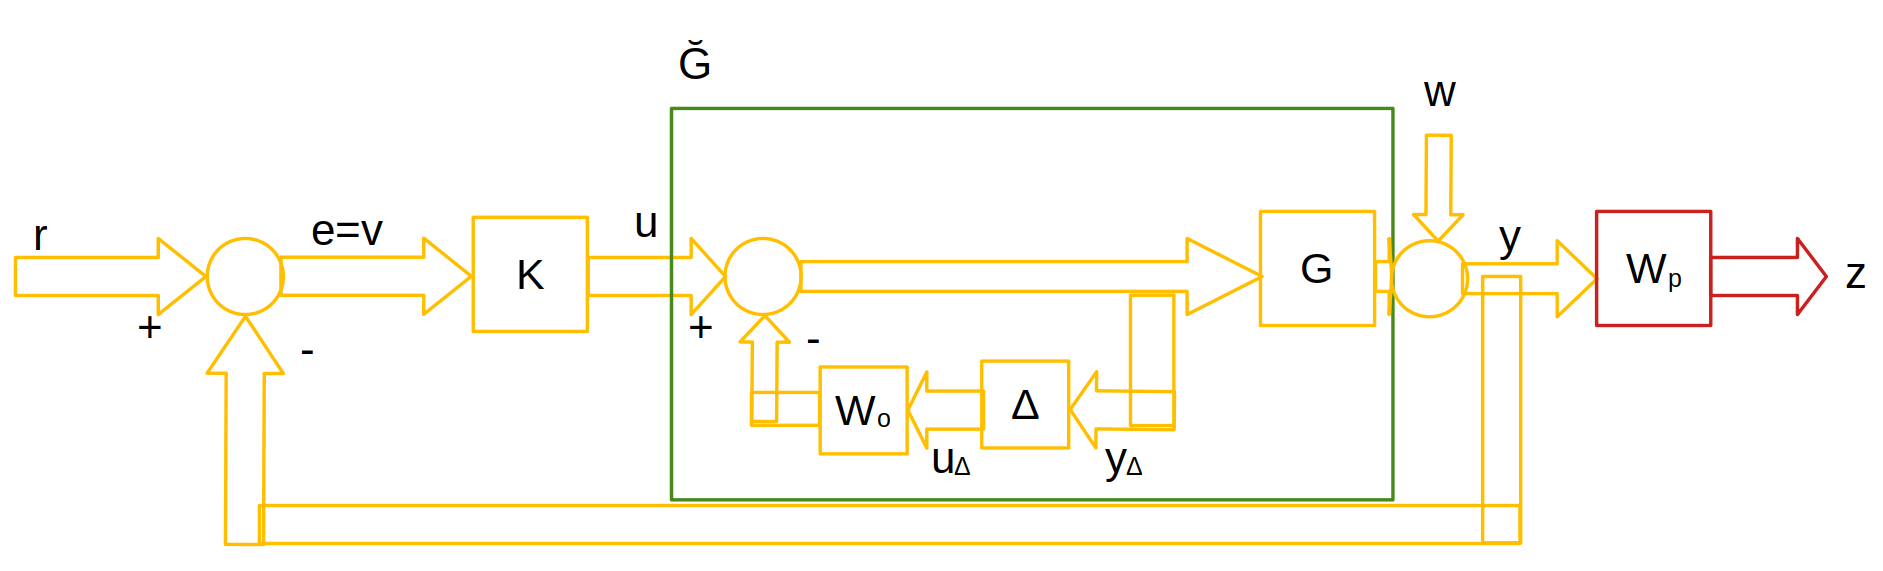
\includegraphics[width=\textwidth]{1blockDiagram.png}
    \caption{Block diagram of the overall system with labeled components.}
    \label{fig:1blockDiagram}
\end{figure}

\subsection{} 
\textit{Compute the generalized plant $P$ and close the lower LFT (with $\Delta \neq 0$) to compute $N$. What are the corresponding tests for nominal performance and robust stability?}

Writing $y_{\Delta}$, $v$, $z$ in terms of $u_{\Delta}$, $w$, $u$:

\begin{align*}
    y_{\Delta} &= u - W_o u_{\Delta} \\
    z &= W_p(w + G(u - u_{\Delta})) \\
    v &= -y \\
      &= -w -G(u-u_{\Delta}) \\
\end{align*}

\[
\begin{bmatrix}
    y_{\Delta} \\
    z \\
    v
\end{bmatrix}
=
\begin{bmatrix}
    -W_o & 0 & I \\
    -W_p G & W_p & W_p G \\
    G & -I & -G
\end{bmatrix}
\begin{bmatrix}
    u_{\Delta} \\
    w \\
    u
\end{bmatrix}
\]

Closing lower LFT:
\begin{align*}
    N = F_l(P,K) &= P_{11} + P_{12} K (I - P_{22} K)^{-1} P_{21} \\
    &= \begin{bmatrix} -W_o & 0 \\ -W_p G & W_p \end{bmatrix} + \begin{bmatrix} I \\ W_p G \end{bmatrix} K (I - G K)^{-1} \begin{bmatrix} G & -I \end{bmatrix} \\
    &= \begin{bmatrix} -W_o + K (I - G K)^{-1} G & -K (I - G K)^{-1} \\ -W_p G + W_p G K (I - G K)^{-1} G & W_p - W_p G K (I - G K)^{-1} \end{bmatrix} \\
    &= \begin{bmatrix} -W_o + T_I & -K S_O \\ W_p G S_O & W_p S_O \end{bmatrix} \\
\end{align*}

The test for robust stability is comes from the $N_{11}$ block so $-W_o + T_I$.
The test for nominal performance comes from the $N_{22}$ block so $W_p S_O$.
Need those $H_\infty$ norms to be less than 1.

\subsection{} 
\textit{Assume a performance weighting function to be $W_p(s) = w_p(s) I$ where $w_p(s) = (s / M + \omega_B^*)/(s + \omega_B^* A)$, with $A = 4$; $M = 10$; $\omega_B^* = 3$. Does the system satisfy this nominal performance criterion you derived in part (b)?}

\subsection{} 
\textit{Assume an uncertainty weighting function to be $W_o(s) = w_o(s) I$ where $w_o(s) = (\tau s + r_0)/(\tau s / r_{\infty} + 1)$, with $\tau = 0.02$, $r_0 = 0.05$, $r_{\infty} = 0.4$, and full (unstructured) uncertainty. Is the system robustly stable using the criterion you derived in part (b)?}

\textit{Hint: to compute the state space model for the controller, assume $D = K$ (static gain) and the $A, B, C$ matrices are all zeros with appropriate dimensions.}

\end{document}